\paragraph*{Learned cross-resource allocation under mixed disturbances.}
The supplementary attention analysis makes the interaction patterns behind the heterogeneous representation visible (Figures~\ref{fig:attn-change} and \ref{fig:attn-types}). It uses the \texttt{dense\_i1\_mix\_start5\_min8\_cause4\_opt\_main\_seed42} checkpoint, with 96 test samples per condition selected deterministically with episode stratification. Normal samples have neither a current nor a future bottleneck; upcoming samples have no current bottleneck but at least one future bottleneck; ongoing samples have at least one current bottleneck. Resource weights are averaged over samples, history steps, heads and encoder layers, with dropout inactive. For readability, all resource-level heatmaps display the 20 machine, gantry, human and AGV nodes and omit the 18 buffer rows and columns without renormalizing the retained values. The corresponding absolute matrices are retained in Appendix~\ref{app:absolute-attention}.

Subtracting the normal-condition average in Figure~\ref{fig:attn-change} removes the persistent attention backbone and exposes the localized redistribution associated with upcoming and ongoing bottlenecks. The type-level summary in Figure~\ref{fig:attn-types} makes interactions among machines, gantries, humans and AGVs easier to inspect. Each cell is a mean over a query-type/attended-type block, not the total attention mass assigned to that type; group sizes differ. These views describe how heterogeneous information is used in the supplementary checkpoints. The configuration comparisons above, rather than attention magnitude, quantify predictive benefit.

\begin{figure*}[t]
\centering
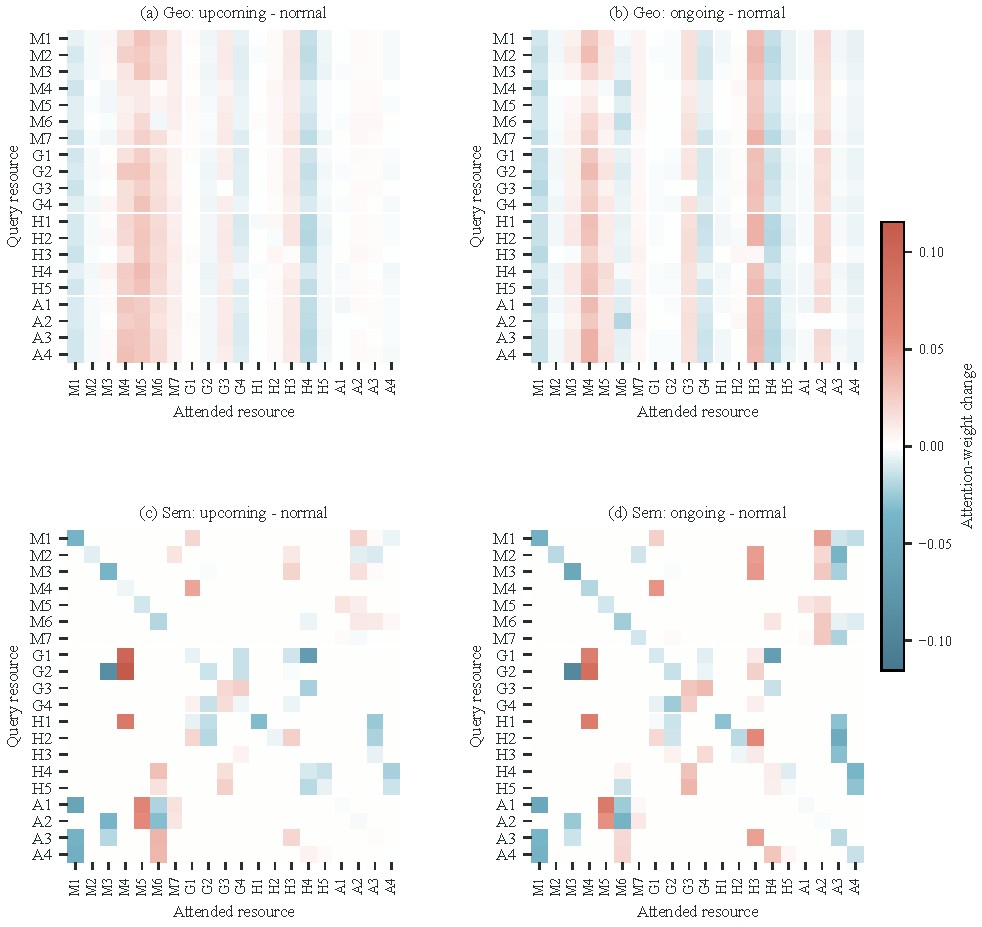
\includegraphics[width=0.92\textwidth]{figures/attention_heatmaps/fig03_resource_attention_change.pdf}
\caption{Resource-attention redistribution relative to normal for upcoming and ongoing samples (coral: increase; blue: decrease).}
\label{fig:attn-change}
\end{figure*}
\begin{figure*}[t]
\centering
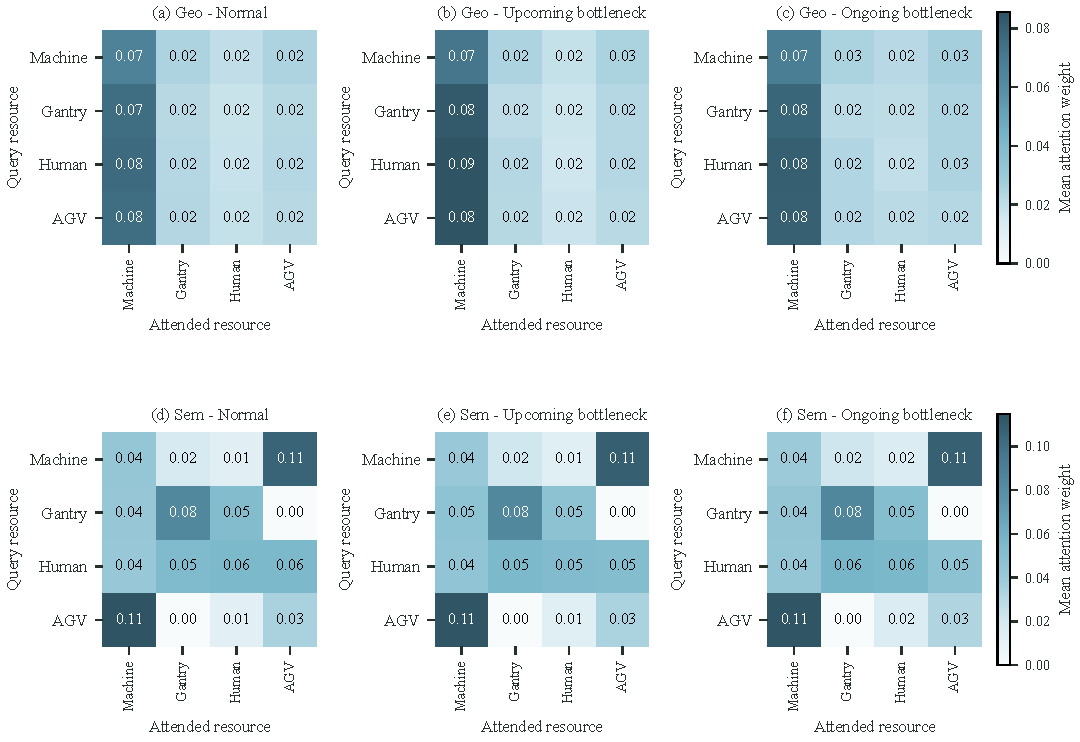
\includegraphics[width=0.92\textwidth]{figures/attention_heatmaps/fig06_entity_type_attention.pdf}
\caption{Type-level attention summary under normal, upcoming, and ongoing conditions (buffers omitted).}
\label{fig:attn-types}
\end{figure*}
